\documentclass[12pt,a4paper]{article}

% -------------------------------------------------
% PACKAGES (LaTeX equivalent of Word features)
% -------------------------------------------------
\usepackage[utf8]{inputenc}
\usepackage[T1]{fontenc}
\usepackage[ngerman,english]{babel}
\usepackage{geometry}
\usepackage{graphicx}
\usepackage{float}        % for [H] figure placement (use sparingly)
\usepackage{caption}      % better caption control
\usepackage{booktabs}     % nicer tables
\usepackage{longtable}    % tables over page breaks
\usepackage{array}        % column width control
\usepackage{enumitem}     % compact lists
\usepackage{fancyhdr}     % headers/footers
\usepackage{hyperref}     % hyperlinks + clickable refs
\usepackage{amssymb}      % for \boxtimes checkbox (see source comment below)

\geometry{margin=2.5cm}

% -------------------------------------------------
% HEADER / FOOTER
% -------------------------------------------------
\pagestyle{fancy}
\fancyhf{}
\fancyfoot[C]{\thepage}
\renewcommand{\headrulewidth}{0pt}

\hypersetup{
  colorlinks=true,
  linkcolor=black,
  urlcolor=blue
}

% -------------------------------------------------
\newcommand{\checkedbox}{\(\boxtimes\)}
\newcommand{\uncheckedbox}{\(\square\)}

% -------------------------------------------------
% FIX FORMATTING OF SMALL TITLES + LISTS + HYPHENATION
% -------------------------------------------------

% Mini heading: consistent spacing + forces following text to start flush-left
\newcommand{\minititle}[1]{%
  \par\addvspace{0.6\baselineskip}%
  \noindent\textbf{#1}\par\nobreak%
  \noindent\ignorespaces%
}

% Make itemize/enumerate look cleaner (less indent, better spacing)
\setlist[itemize]{leftmargin=*, topsep=0.35\baselineskip, itemsep=0.15\baselineskip, parsep=0pt}
\setlist[enumerate]{leftmargin=*, topsep=0.35\baselineskip, itemsep=0.15\baselineskip, parsep=0pt}

% Reduce ugly hyphenation like "archi-tectural"
\setlength{\emergencystretch}{2em}

% -------------------------------------------------
\begin{document}

% =========================================================
% PAGE 1: TITLE PAGE 
% =========================================================
\begin{titlepage}
\thispagestyle{empty}

% move header up
\vspace*{-2.5cm}

\noindent
\begin{minipage}[t]{0.45\textwidth}
  \raggedright
  
\includegraphics[height=1.3cm]{HSLU LOGO.png}
\end{minipage}
\hfill
\begin{minipage}[t]{0.45\textwidth}
  \hspace*{1cm}% move right
  
\includegraphics[height=1.2cm]{INFORMATIK.png}
\end{minipage}

    %Hier ein aussagekräftiger Titel und beide Autoren. Eventuell ein illustrierendes Bild.\\ Ansonsten ist diese erste Seite bzw. Frontseite frei gestaltbar.

    % --- This reproduces the big empty space in the Word template ---
    \vspace*{9cm}

    \begin{center}
        {\Huge \textbf{Titel der Transferarbeit}}\\[0.8cm]
        {\Large \textit{Autoren}}\\[1.5cm]
        \vfill
    \end{center}
\end{titlepage}

% =========================================================
% PAGE 2: FORMAL INFO + DECLARATION + LINK 
% =========================================================
\newpage
\thispagestyle{empty}

\begin{center}
{\Large \textbf{Transferarbeit an der Hochschule Luzern – Informatik}}
\end{center}

\vspace{1cm}

\noindent
\textbf{Titel:} 

\vspace{0.6cm}

\noindent
\textbf{Teilnehmerin/Teilnehmer:} 

\vspace{0.6cm}

\noindent
\textbf{Teilnehmerin/Teilnehmer:} 

\vspace{0.8cm}

\noindent
\textbf{Programm:} CAS Software Architecture

\vspace{0.6cm}

\noindent
\textbf{Zeitraum:}

\vspace{0.8cm}

\noindent
\textbf{Programmleitung:} Prof.\ Dr.\ habil.\ Jana Koehler, Dr.\ Stefan Bischoff

\vspace{0.6cm}

\noindent
\textbf{Betreuung/Referat:} 

\vspace{1.2cm}

\noindent
\textbf{Codierung / Klassifizierung der Arbeit:}

\vspace{0.4cm}

\noindent
\checkedbox\ Öffentlich (Normalfall)

\noindent
\uncheckedbox\ Vertraulich

\vspace{1.2cm}

\noindent
\textbf{Eidesstattliche Erklärung}

\vspace{0.4cm}

\noindent
Ich erkläre hiermit, dass ich/wir die vorliegende Arbeit selbständig und ohne unerlaubte fremde Hilfe angefertigt haben, alle verwendeten Quellen, Literatur und andere Hilfsmittel angegeben haben, wörtlich oder inhaltlich entnommene Stellen als solche kenntlich gemacht haben, das Vertraulichkeitsinteresse des Auftraggebers wahren und die Urheberrechtsbestimmungen der Hochschule Luzern respektieren werden.

\vspace{1.4cm}

\noindent
Ort / Datum, Unterschrift \hspace{0.7em}\rule{10.2cm}{0.4pt}

\vspace{1.0cm}

\noindent
Ort / Datum, Unterschrift \hspace{0.7em}\rule{10.2cm}{0.4pt}

\vspace{1.6cm}

\noindent
Geistiges Eigentum gemäss der
\href{https://srl.lu.ch/app/de/texts_of_law/521/versions/3884}{Studienordnung}
für die Ausbildung an der Hochschule Luzern, FH Zentralschweiz

% =========================================================
% PREFACE TEXT 
% =========================================================
\newpage
\pagenumbering{arabic}

\noindent
% Das folgende Template ist im Wesentlichen von arc42 übernommen. Bitte passt es an entsprechend Eurer Arbeitsschwerpunkte, unseren Pflichtinhalten und den Methoden, die wir im Kurs verwenden. Ich habe auch noch einige zusätzliche Kommentare hinzugefügt, die erklären was wir in den einzelnen Kapiteln an Inhalten gerne sehen würden. Seitenzahlen sind eingefügt und in der Fusszeile sichtbar. Sollten hier Probleme bei Euch auftreten, schaut in Word unter Einfügen > Fusszeile bearbeiten und stellt sicher, dass «Mit vorheriger verknüpfen» aktiviert ist. Ihr könnt gerne die Seitenzahlen auch an einer anderen Position platzieren, z.B. in der Kopfzeile, wenn es Euch besser gefällt.

\vspace{1cm}

% =========================================================
% TABLE OF CONTENTS / LIST OF FIGURES
% =========================================================
\tableofcontents
\newpage

\listoffigures
\newpage

% -------------------------------------------------
% NOTE ON FIGURES & REFERENCES 
% -------------------------------------------------
% Use captions for figures in a way such that they are automatically maintained by LaTeX.
% In Word this is "Referenzen > Beschriftung einfügen".
% In LaTeX you do this with:
%   \begin{figure} ... \caption{...}\label{fig:xyz}\end{figure}
% and refer to it with:
%   Figure~\ref{fig:xyz}
%
% Hier ein Beispiel für eine Referenz, die dann auch automatisch aktualisiert:
% In Figure~\ref{fig:iso25010}, we discuss …
% (In Word: Einfügen > Querverweis)
%
% Example figure block (upload the image file into Overleaf):
% \begin{figure}[H]
%   \centering
%   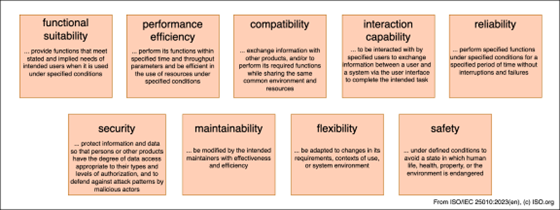
\includegraphics[width=0.9\textwidth]{iso25010.png}
%   \caption{Overview on ISO 25010}
%   \label{fig:iso25010}
% \end{figure}

% =========================================================
% 1. INTRODUCTION AND GOALS
% =========================================================
\section{Introduction and Goals}

Describes the relevant requirements and the driving forces that software architects and development team must consider. These include
\begin{itemize}
  \item underlying business goals,
  \item essential features,
  \item essential functional requirements,
  \item quality goals for the architecture and
  \item relevant stakeholders and their expectations
\end{itemize}

\subsection{Functional Requirements}

\minititle{Contents}
Short description of the functional requirements, driving forces, extract (or abstract) of requirements. Link to (hopefully existing) requirements documents (with version number and information where to find it).

\minititle{Motivation}
From the point of view of the end users a system is created or modified to improve support of a business activity and/or improve the quality.

\minititle{Form}
Short textual description, probably in tabular use-case format. If requirements documents exist this overview should refer to these documents.
Keep these excerpts as short as possible. Balance readability of this document with potential redundancy w.r.t to requirements documents.

\minititle{Further Information}
See Introduction and Goals in the arc42 documentation.

\subsection{Quality Goals}

\minititle{Contents}
The top three (max five) quality goals for the architecture whose fulfillment is of highest importance to the major stakeholders. We really mean quality goals for the architecture. Don’t confuse them with project goals. They are not necessarily identical.
Consider this overview of potential topics (based upon the ISO 25010 standard):

% Figure 1 :
\begin{figure}[H]
  \centering
  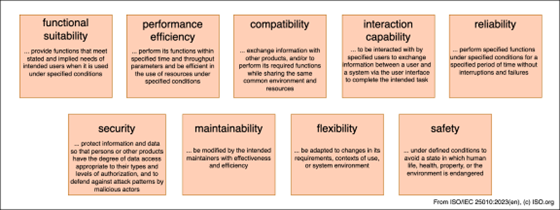
\includegraphics[width=0.85\textwidth]{iso25010.png}
  \caption{Overview on ISO 25010}
  \label{fig:iso25010}
\end{figure}

Hier ein Beispiel für eine Referenz, die dann auch automatisch aktualisiert:

In Figure~\ref{fig:iso25010}, we discuss \dots


\vspace{0.6cm}

\minititle{Motivation}
You should know the quality goals of your most important stakeholders, since they will influence fundamental architectural decisions. Make sure to be very concrete about these qualities, avoid buzzwords. If you as an architect do not know how the quality of your work will be judged\ldots

\minititle{Form}
A table with quality goals and concrete scenarios, ordered by priorities

\subsection{Stakeholders}

% Additional course comment:
% Add the stakeholder power matrix, and/or focus on change management if this is in the focus of your work.
% In any case, some description about the stakeholder universe should be added here.

\minititle{Contents}
Explicit overview of stakeholders of the system, i.e. all person, roles or organizations that
\begin{itemize}
  \item should know the architecture
  \item have to be convinced of the architecture
  \item have to work with the architecture or with code
  \item need the documentation of the architecture for their work
  \item have to come up with decisions about the system or its development
\end{itemize}

\minititle{Motivation}
You should know all parties involved in development of the system or affected by the system. Otherwise, you may get nasty surprises later in the development process. These stakeholders determine the extent and the level of detail of your work and its results.

\minititle{Form}
Table with role names, person names, and their expectations with respect to the architecture and its documentation.

\begin{longtable}{p{3cm} p{4cm} p{7cm}}
\toprule
Role/Name & Contact & Expectations \\
\midrule
\textless Role-1\textgreater & \textless Contact-1\textgreater & \textless Expectation-1\textgreater \\
\textless Role-2\textgreater & \textless Contact-2\textgreater & \textless Expectation-2\textgreater \\
\bottomrule
\end{longtable}

% =========================================================
% 2. ARCHITECTURE CONSTRAINTS
% =========================================================
\section{Architecture Constraints}

\minititle{Contents}
Any requirement that constraints software architects in their freedom of design and implementation decisions or decision about the development process. These constraints sometimes go beyond individual systems and are valid for whole organizations and companies.

\minititle{Motivation}
Architects should know exactly where they are free in their design decisions and where they must adhere to constraints. Constraints must always be dealt with; they may be negotiable, though.

\minititle{Form}
Simple tables of constraints with explanations. If needed you can subdivide them into technical constraints, organizational and political constraints and conventions (e.g. programming or versioning guidelines, documentation or naming conventions)

\minititle{Further Information}
See Architecture Constraints in the arc42 documentation:
\href{https://docs.arc42.org/section-2/}{https://docs.arc42.org/section-2/}

% =========================================================
% 3. CONTEXT AND SCOPE
% =========================================================
\section{Context and Scope}

\minititle{Contents}
Context and scope - as the name suggests - delimits your system (i.e. your scope) from all its communication partners (neighboring systems and users, i.e. the context of your system). It thereby specifies the external interfaces.
If necessary, differentiate the business context (domain specific inputs and outputs) from the technical context (channels, protocols, hardware).

\minititle{Motivation}
The domain interfaces and technical interfaces to communication partners are among your system’s most critical aspects. Make sure that you completely understand them.

\minititle{Form}
Various options:
\begin{itemize}
  \item Context diagrams
  \item Lists of communication partners and their interfaces.
\end{itemize}

\minititle{Further Information}
See Context and Scope in the arc42 documentation:
\href{https://docs.arc42.org/section-3/}{https://docs.arc42.org/section-3/}

\subsection{Business Context}

\minititle{Contents}
Specification of all communication partners (users, IT-systems, \dots) with explanations of domain specific inputs and outputs or interfaces. Optionally you can add domain specific formats or communication protocols.

\minititle{Motivation}
All stakeholders should understand which data are exchanged with the environment of the system.

\minititle{Form}
All kinds of diagrams that show the system as a black box and specify the domain interfaces to communication partners.
Alternatively (or additionally) you can use a table. The title of the table is the name of your system, the three columns contain the name of the communication partner, the inputs, and the outputs.
\textless Diagram or Table\textgreater\\
\textless optionally: Explanation of external domain interfaces\textgreater

\subsection{Technical Context}

\minititle{Contents}
Technical interfaces (channels and transmission media) linking your system to its environment. In addition a mapping of domain specific input/output to the channels, i.e. an explanation which I/O uses which channel.

\minititle{Motivation}
Many stakeholders make architectural decision based on the technical interfaces between the system and its context. Especially infrastructure or hardware designers decide these technical interfaces.

\minititle{Form}
E.g. UML deployment diagram describing channels to neighboring systems, together with a mapping table showing the relationships between channels and input/output.
\textless Diagram or Table\textgreater\\
\textless optionally: Explanation of technical interfaces\textgreater\\
\textless Mapping Input/Output to Channels\textgreater

% =========================================================
% 4. SOLUTION STRATEGY
% =========================================================
\section{Solution Strategy}

\minititle{Contents}
A short summary and explanation of the fundamental decisions and solution strategies, that shape system architecture. It includes
\begin{itemize}
  \item technology decisions
  \item decisions about the top-level decomposition of the system, e.g. usage of an architectural pattern or design pattern
  \item decisions on how to achieve key quality goals
  \item relevant organizational decisions, e.g. selecting a development process or delegating certain tasks to third parties.
\end{itemize}

\minititle{Motivation}
These decisions form the cornerstones for your architecture. They are the foundation for many other detailed decisions or implementation rules.

\minititle{Form}
Keep the explanations of such key decisions short.\\
Motivate what was decided and why it was decided that way, based upon problem statement, quality goals and key constraints. Refer to details in the following sections.

% Course comment:
% Define your selected principles, discuss chosen architectural style,
% use templates for architectural decisions (which follow in detail in Chapter 9).
% Do not forget the context view (in this chapter or before Chapter 5 in a separate chapter)

\minititle{Further Information}
See Solution Strategy in the arc42 documentation:
\href{https://docs.arc42.org/section-4/}{https://docs.arc42.org/section-4/}

% =========================================================
% 5. BUILDING BLOCK VIEW
% =========================================================
\section{Building Block View}

\minititle{Content}
The building block view shows the static decomposition of the system into building blocks (modules, components, subsystems, classes, interfaces, packages, libraries, frameworks, layers, partitions, tiers, functions, macros, operations, data structures, \dots) as well as their dependencies (relationships, associations, \dots)\\
This view is mandatory for every architecture documentation. In analogy to a house this is the floor plan.

\minititle{Motivation}
Maintain an overview of your source code by making its structure understandable through abstraction.
This allows you to communicate with your stakeholder on an abstract level without disclosing implementation details.
\minititle{Form}
The building block view is a hierarchical collection of black boxes and white boxes (see figure below) and their descriptions.
% Figure 2 :
\begin{figure}[H]
  \centering
  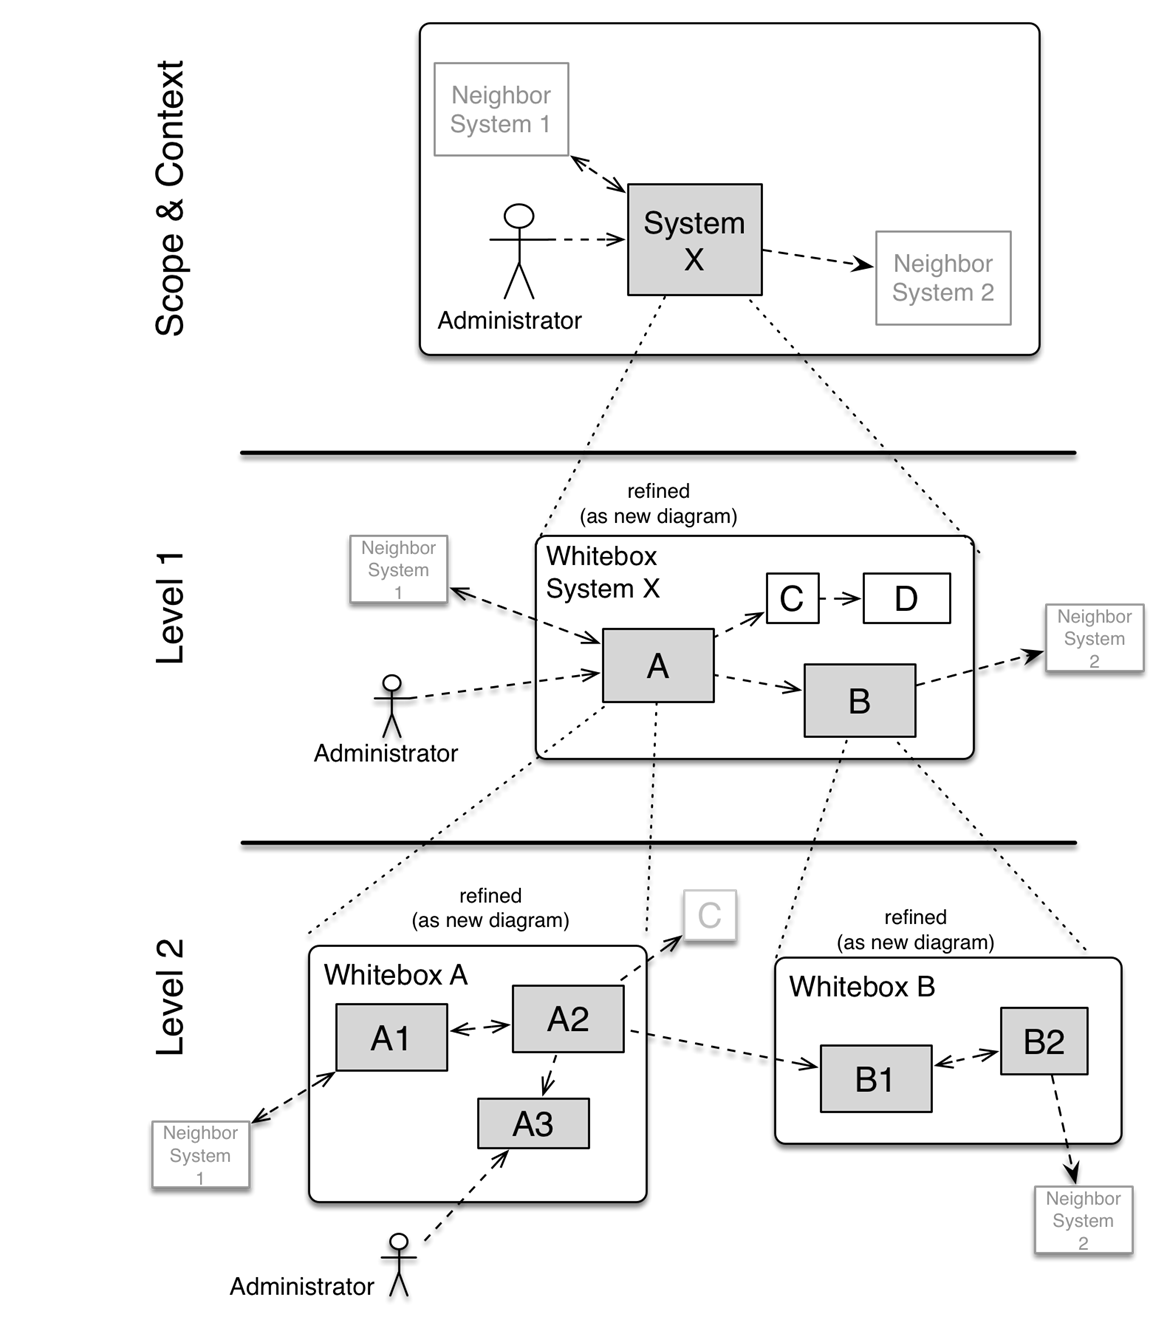
\includegraphics[width=0.85\textwidth]{building-block-view-example.png}
  \caption{Example for Building Block View from template (hint: rather use clean UML package or component diagrams)}
  \label{fig:bbv-example}
\end{figure}

Level 1 is the white box description of the overall system together with black box descriptions of all contained building blocks.
Level 2 zooms into some building blocks of level 1. Thus it contains the white box description of selected building blocks of level 1, together with black box descriptions of their internal building blocks.
Level 3 zooms into selected building blocks of level 2, and so on.

\minititle{Further Information}
See Building Block View in the arc42 documentation:
\href{https://docs.arc42.org/section-5/}{https://docs.arc42.org/section-5/}

\subsection{Whitebox Overall System}

Here you describe the decomposition of the overall system using the following white box template. It contains
\begin{itemize}
  \item an overview diagram
  \item a motivation for the decomposition
  \item black box descriptions of the contained building blocks. For these we offer you alternatives:
    \begin{itemize}
      \item use one table for a short and pragmatic overview of all contained building blocks and their interfaces
      \item use a list of black box descriptions of the building blocks according to the black box template (see below). Depending on your choice of tool this list could be sub-chapters (in text files), sub-pages (in a Wiki) or nested elements (in a modeling tool).
    \end{itemize}
  \item (optional:) important interfaces, that are not explained in the black box templates of a building block, but are very important for understanding the white box. Since there are so many ways to specify interfaces why do not provide a specific template for them. In the worst case you have to specify and describe syntax, semantics, protocols, error handling, restrictions, versions, qualities, necessary compatibilities and many things more. In the best case you will get away with examples or simple signatures.
\end{itemize}

\textless Overview Diagram\textgreater

\subsubsection*{Motivation}
\textless text explanation\textgreater

\subsubsection*{Contained Building Blocks}
\textless Description of contained building block (black boxes)\textgreater

\subsubsection*{Important Interfaces}
\textless Description of important interfaces\textgreater
Insert your explanations of black boxes from level 1:
If you use tabular form you will only describe your black boxes with name and responsibility according to the following schema:

\begin{table}[H]
\centering
\begin{tabular}{p{4cm} p{9cm}}
\toprule
Name & Responsibility \\
\midrule
\textless black box 1\textgreater & \textless Text\textgreater \\
\textless black box 2\textgreater & \textless Text\textgreater \\
\bottomrule
\end{tabular}
\caption{Contained Building Blocks (Level 1)}
\end{table}
If you use a list of black box descriptions then you fill in a separate black box template for every important building block. Its headline is the name of the black box.

\subsubsection{\textless Name black box 1\textgreater}

Here you describe \textless black box 1\textgreater\ according the the following black box template:
\begin{itemize}
  \item Purpose/Responsibility
  \item Interface(s), when they are not extracted as separate paragraphs. This interfaces may include qualities and performance characteristics.
  \item (Optional) Quality-/Performance characteristics of the black box, e.g. availability, run time behavior, \dots
  \item (Optional) directory/file location
  \item (Optional) Fulfilled requirements (if you need traceability to requirements).
  \item (Optional) Open issues/problems/risks
\end{itemize}

\textless Purpose/Responsibility\textgreater

\textless Interface(s)\textgreater

\textless (Optional) Quality/Performance Characteristics\textgreater

\textless (Optional) Directory/File Location\textgreater

\textless (Optional) Fulfilled Requirements\textgreater

\textless (Optional) Open Issues/Problems/Risks\textgreater

\subsubsection{\textless Name black box 2\textgreater}
\textless black box template\textgreater

\subsubsection{\textless Name black box n\textgreater}
\textless black box template\textgreater

\subsubsection{\textless Name interface 1\textgreater}
\dots

\subsubsection{\textless Name interface m\textgreater}
\dots

\subsection{Level 2}

Here you can specify the inner structure of (some) building blocks from level 1 as white boxes.

You have to decide which building blocks of your system are important enough to justify such a detailed description. Please prefer relevance over completeness. Specify important, surprising, risky, complex or volatile building blocks. Leave out normal, simple, boring or standardized parts of your system

\subsubsection{White Box \textless building block 1\textgreater}
\dots describes the internal structure of building block 1.\\
\textless white box template\textgreater

\subsubsection{White Box \textless building block 2\textgreater}
\textless white box template\textgreater

\subsubsection{White Box \textless building block m\textgreater}
\textless white box template\textgreater

\subsection{Level 3}

Here you can specify the inner structure of (some) building blocks from level 2 as white boxes.

When you need more detailed levels of your architecture please copy this part of arc42 for additional levels.

\subsubsection{White Box \textless\_building block x.1\_\textgreater}
Specifies the internal structure of building block x.1.\\
\textless white box template\textgreater

\subsubsection{White Box \textless\_building block x.2\_\textgreater}
\textless white box template\textgreater

\subsubsection{White Box \textless\_building block y.1\_\textgreater}
\textless white box template\textgreater

% =========================================================
% 6. RUNTIME VIEW
% =========================================================
\section{Runtime View}

\minititle{Contents}
The runtime view describes concrete behavior and interactions of the system’s building blocks in form of scenarios from the following areas:
\begin{itemize}
  \item important use cases or features: how do building blocks execute them?
  \item interactions at critical external interfaces: how do building blocks cooperate with users and neighboring systems?
  \item operation and administration: launch, start-up, stop
  \item error and exception scenarios
\end{itemize}

\noindent\textbf{Remark:} The main criterion for the choice of possible scenarios (sequences, workflows) is their architectural relevance. It is not important to describe a large number of scenarios. You should rather document a representative selection.

\minititle{Motivation}
You should understand how (instances of) building blocks of your system perform their job and communicate at runtime. You will mainly capture scenarios in your documentation to communicate your architecture to stakeholders that are less willing or able to read and understand the static models (building block view, deployment view).

\minititle{Form}
There are many notations for describing scenarios, e.g.
\begin{itemize}
  \item numbered list of steps (in natural language)
  \item activity diagrams or flow charts
  \item sequence diagrams
  \item BPMN or EPCs (event process chains)
  \item state machines
  \item \dots
\end{itemize}

\minititle{Further Information}
See Runtime View in the arc42 documentation:
\href{https://docs.arc42.org/section-6/}{https://docs.arc42.org/section-6/}

\subsection{\textless Runtime Scenario 1\textgreater}
\begin{itemize}
  \item \textless insert runtime diagram or textual description of the scenario\textgreater
  \item \textless insert description of the notable aspects of the interactions between the building block instances depicted in this diagram\textgreater
\end{itemize}

\subsection{\textless Runtime Scenario 2\textgreater}
\dots

\subsection{\textless Runtime Scenario n\textgreater}
\dots

% =========================================================
% 7. DEPLOYMENT VIEW
% =========================================================
\section{Deployment View}

\minititle{Content}
The deployment view describes:
\begin{enumerate}
  \item technical infrastructure used to execute your system, with infrastructure elements like geographical locations, environments, computers, processors, channels and net topologies as well as other infrastructure elements and
  \item mapping of (software) building blocks to that infrastructure elements.
\end{enumerate}

Often systems are executed in different environments, e.g. development environment, test environment, production environment. In such cases you should document all relevant environments.

Especially document a deployment view if your software is executed as distributed system with more than one computer, processor, server or container or when you design and construct your own hardware processors and chips.

From a software perspective it is sufficient to capture only those elements of an infrastructure that are needed to show a deployment of your building blocks. Hardware architects can go beyond that and describe an infrastructure to any level of detail they need to capture.

\minititle{Motivation}
Software does not run without hardware. This underlying infrastructure can and will influence a system and/or some cross-cutting concepts. Therefore, there is a need to know the infrastructure.

\minititle{Form}
Maybe a highest level deployment diagram is already contained in section 3.2. as technical context with your own infrastructure as ONE black box. In this section one can zoom into this black box using additional deployment diagrams:
\begin{itemize}
  \item UML offers deployment diagrams to express that view. Use it, probably with nested diagrams, when your infrastructure is more complex.
  \item When your (hardware) stakeholders prefer other kinds of diagrams rather than a deployment diagram, let them use any kind that is able to show nodes and channels of the infrastructure.
\end{itemize}

\minititle{Further Information}
See Deployment View in the arc42 documentation:
\href{https://docs.arc42.org/section-7/}{https://docs.arc42.org/section-7/}

\subsection{Infrastructure Level 1}

Describe (usually in a combination of diagrams, tables, and text):
\begin{itemize}
  \item distribution of a system to multiple locations, environments, computers, processors, \dots, as well as physical connections between them
  \item important justifications or motivations for this deployment structure
  \item quality and/or performance features of this infrastructure
  \item mapping of software artifacts to elements of this infrastructure
\end{itemize}

For multiple environments or alternative deployments please copy and adapt this section of arc42 for all relevant environments.

\textless Overview Diagram\textgreater

\subsubsection*{Motivation}
\textless explanation in text form\textgreater

\subsubsection*{Quality and/or Performance Features}
\textless explanation in text form\textgreater

\subsubsection*{Mapping of Building Blocks to Infrastructure}
\textless description of the mapping\textgreater

\subsection{Infrastructure Level 2}

Here you can include the internal structure of (some) infrastructure elements from level 1.

Please copy the structure from level 1 for each selected element.

\subsubsection{\textless Infrastructure Element 1\textgreater}
\textless diagram + explanation\textgreater

\subsubsection{\textless Infrastructure Element 2\textgreater}
\textless diagram + explanation\textgreater

\subsubsection{\textless Infrastructure Element n\textgreater}
\textless diagram + explanation\textgreater

% =========================================================
% 8. CROSS-CUTTING CONCEPTS
% =========================================================
\section{Cross-cutting Concepts}

\minititle{Content}
This section describes crosscutting concepts (practices, patterns, regulations or solution ideas). Such concepts are often related to multiple building blocks. They may include many different topics, such as the topics shown in the following diagram:

% Figure 3:
\begin{figure}[H]
  \centering
  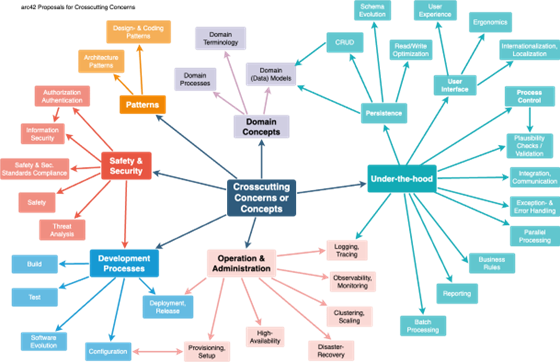
\includegraphics[width=0.85\textwidth]{cross-cutting-concerns.png}
  \caption{Chaotic Cross-Cutting Concerns in arc42, Domain Concepts etc. belong into a DDD subchapter, Safety, Security, under-the hood are quality categories in ISO 25010 (clean this up for your project).}
  \label{fig:ccc}
\end{figure}

% Additional course comment:
% Carefully think if your planned content here does not better belong into the other chapters!!!
% Development issues can be discussed here, but deployment belongs to the operational model.
% Similarly, most of the under-the-hood entries either belong into the ADM,
% or the quality discussion, or process model analysis and modeling.

\minititle{Motivation}
Concepts form the basis for conceptual integrity (consistency, homogeneity) of the architecture. Thus, they are an important contribution to achieve inner qualities of your system.

This is the place in the template that we provided for a cohesive specification of such concepts.

Many of these concepts relate to or influence several of your building blocks.

\minititle{Form}
The form can be varied:
\begin{itemize}
  \item concept papers with any kind of structure
  \item example implementations, especially for technical concepts
  \item cross-cutting model excerpts or scenarios using notations of the architecture views
\end{itemize}

\minititle{Structure}
Pick only the most-needed topics for your system and assign each a level-2 heading in this section (e.g. 8.1, 8.2 etc).

DO NOT ATTEMPT to cover all of the topics of the aforementioned diagram.

\minititle{Further Information}
See Concepts in the arc42 documentation:
\href{https://docs.arc42.org/section-8/}{https://docs.arc42.org/section-8/}

\subsection{\textless Concept 1\textgreater}
\textless explanation\textgreater

\subsection{\textless Concept 2\textgreater}
\textless explanation\textgreater

\subsection{\textless Concept n\textgreater}
\textless explanation\textgreater

% =========================================================
% 9. ARCHITECTURE DECISIONS
% =========================================================
\section{Architecture Decisions}

\minititle{Contents}
Important, expensive, large scale or risky architecture decisions including rationales. With ``decisions'' we mean selecting one alternative based on given criteria.

Please use your judgement to decide whether an architectural decision should be documented here in this central section or whether you better document it locally (e.g. within the white box template of one building block).

Avoid redundancy. Refer to section 4, where you already captured the most important decisions of your architecture.

\minititle{Motivation}
Stakeholders of your system should be able to comprehend and retrace your decisions.

\minititle{Form}
Various options:
\begin{itemize}
  \item ADR (Documenting Architecture Decisions) for every important decision
  \item List or table, ordered by importance and consequences or:
  \item more detailed in form of separate sections per decision
\end{itemize}

% Course comment:
% Use 1 template (and explain why you chose this particular one), add a reference to the template.
% Make sure your ADR are SMART.

\minititle{Further Information}
See Architecture Decisions in the arc42 documentation:
\href{https://docs.arc42.org/section-9/}{https://docs.arc42.org/section-9/}\\
Documenting Architecture Decisions (ADR):\\
\href{https://cognitect.com/blog/2011/11/15/documenting-architecture-decisions}{https://cognitect.com/blog/2011/11/15/documenting-architecture-decisions}

% =========================================================
% 10. QUALITY REQUIREMENTS
% =========================================================
\section{Quality Requirements}

\minititle{Content}
This section contains all relevant quality requirements.

The most important of these requirements have already been described in section 1.2. (quality goals), therefore they should only be referenced here. In this section 10 you should also capture quality requirements with lesser importance, which will not create high risks when they are not fully achieved (but might be nice-to-have).

\minititle{Motivation}
Since quality requirements will have a lot of influence on architectural decisions you should know what qualities are really important for your stakeholders, in a specific and measurable way.

\begin{itemize}
  \item See Quality Requirements in the arc42 documentation:
  \href{https://docs.arc42.org/section-10/}{https://docs.arc42.org/section-10/}
  \item See the extensive Q42 quality model on \href{https://quality.arc42.org/}{https://quality.arc42.org}
\end{itemize}

% Course comment:
% Write scenarios refining the top quality attributes.

\subsection{Quality Requirements Overview}

\minititle{Content}
An overview or summary of quality requirements.

\minititle{Motivation}
Often we encounter dozens (or even hundreds) of detailed quality requirements. In this overview section you should try to summarize, e.g. by describing categories or topics (as suggested by ISO 25010:2023 or Q42)

If these summary descriptions are already precise, specific enough and measurable, you may skip section 10.2.

\minititle{Form}
Use a simple table in which each line contains a category or topic and a short description of the quality requirement. Alternatively, you may use a mindmap to structure these quality requirements. In literature, the idea of a quality attribute tree has also been described, which puts the generic term ``quality'' as the root and uses a tree-like refinement of the term ``quality''. [Bass+21] introduced the term ``Quality Attribute Utility Tree'' for this purpose.

\subsection{Quality Scenarios}

\minititle{Content}
Quality scenarios make quality requirements concrete and allow to decide whether they are fulfilled (in the sense of acceptance criteria). Ensure that your scenarios are specific and measurable.

Two kinds of scenarios are especially useful:
\begin{itemize}
  \item Usage scenarios (also called application scenarios or use case scenarios) describe the system’s runtime reaction to a certain stimulus. This also includes scenarios that describe the system’s efficiency or performance. Example: The system reacts to a user’s request within one second.
  \item Change scenarios describe the desired effect of a modification or extension of the system or of its immediate environment. Example: Additional functionality is implemented or requirements for a quality attribute change, and the effort or duration of the change is measured.
\end{itemize}

\minititle{Form}
Typical information for detailed scenarios include the following:

In short form (favoured in the Q42 model):
\begin{itemize}
  \item Context/Background: What kind of system or component, what is the environment or situation?
  \item Source/Stimulus: Who or what initiates or triggers a behaviour, reaction or action.
  \item Metric/Acceptance Criteria: A response including a measure or metric
\end{itemize}

The long form of scenarios (favoured by the SEI and [Bass+21]) is more detailed and includes the following information:
\begin{itemize}
  \item Scenario ID: A unique identifier for the scenario.
  \item Scenario Name: A short, descriptive name for the scenario.
  \item Source: The entity (user, system, or event) that initiates the scenario.
  \item Stimulus: The triggering event or condition the system must address.
  \item Environment: The operational context or condition under which the system experiences the stimulus.
  \item Artifact: The building-blocks or other elements of the system affected by the stimulus.
  \item Response: The outcome or behavior the system exhibits in reaction to the stimulus.
  \item Response Measure: The criteria or metric by which the system’s response is evaluated.
\end{itemize}

\minititle{Examples}
See the Q42 quality model website for detailed examples of quality requirements:
\href{https://quality.arc42.org/}{https://quality.arc42.org}

% ISO / Q42 links:
ISO 25010: \href{https://www.iso.org/obp/ui/\#iso:std:iso-iec:25010:ed-2:v1:en}{https://www.iso.org/obp/ui/\#iso:std:iso-iec:25010:ed-2:v1:en}\\
Q42: \href{https://quality.arc42.org/}{https://quality.arc42.org/}

% =========================================================
% 11. RISKS AND TECHNICAL DEBTS
% =========================================================
\section{Risks and Technical Debts}

\minititle{Contents}
A list of identified technical risks or technical debts, ordered by priority

\minititle{Motivation}
“Risk management is project management for grown-ups” (Tim Lister, Atlantic Systems Guild.)

This should be your motto for systematic detection and evaluation of risks and technical debts in the architecture, which will be needed by management stakeholders (e.g. project managers, product owners) as part of the overall risk analysis and measurement planning.

\minititle{Form}
List of risks and/or technical debts, probably including suggested measures to minimize, mitigate or avoid risks or reduce technical debts.

\minititle{Further Information}
See Risks and Technical Debt in the arc42 documentation:
\href{https://docs.arc42.org/section-11/}{https://docs.arc42.org/section-11/}

% =========================================================
% 12. GLOSSARY
% =========================================================
\section{Glossary}

\minititle{Contents}
The most important domain and technical terms that your stakeholders use when discussing the system.

You can also see the glossary as source for translations if you work in multi-language teams.

\minititle{Motivation}
You should clearly define your terms, so that all stakeholders
\begin{itemize}
  \item have an identical understanding of these terms
  \item do not use synonyms and homonyms
\end{itemize}

\minititle{Form}
A table with columns \textless Term\textgreater\ and \textless Definition\textgreater.

Potentially more columns in case you need translations.

\minititle{Further Information}
See Glossary in the arc42 documentation:
\href{https://docs.arc42.org/section-12/}{https://docs.arc42.org/section-12/}

\begin{longtable}{p{4cm} p{10cm}}
\toprule
Term & Definition \\
\midrule
\textless Term-1\textgreater & \textless definition-1\textgreater \\
\textless Term-2\textgreater & \textless definition-2\textgreater \\
\bottomrule
\end{longtable}

% =========================================================
% LIST OF REFERENCES 
% =========================================================
\newpage
\section*{List of References}

% Comment:
% I used keys for papers composed of the first letter of the last name of the first 3 authors + the publication year.
% You can also number your literature references.
% I copied from Google Scholar APA style, but added page numbers for journal articles or conference papers.
%
% I have inserted these examples manually. However, in LaTeX you can maintain your references automatically via BibTeX or biblatex.
% (Word equivalent was: Referenzen > Quellen verwalten, Formatvorlage, Literaturverzeichnis)

\begin{thebibliography}{9}

\bibitem{BPK2021}
BPK2021 Bass, Len, Paul Clements, and Rick Kazman. \textit{Software architecture in practice}. Addison-Wesley Professional, 2021.

\bibitem{CZL2008}
CZL2008 Pautasso, Cesare, Olaf Zimmermann, and Frank Leymann. ``Restful web services vs.\ ``big'' web services: making the right architectural decision.'' \textit{Proceedings of the 17th international conference on World Wide Web}. pp.\ 805--814. 2008.

\bibitem{B1987}
B1987 Brooks, Frederik P., and No Silver Bullet. ``Essence and accidents of software engineering.'' \textit{IEEE computer} 20.4 (1987): 10--19.

\end{thebibliography}

\end{document}
